\section{An Extended Application: \\ Cryptographic Protocol Analysis}

	The chase can be used for protocol analysis. A common technique for the analysis
	of protocols involves identifying the \emph{essentially different} runs of
	the protocol. These essentially different protocol runs are analogous to
	minimal models. When a protocol is described using geometric logic, the
	chase can find such minimal models. The protocol can then be analysed for
	characteristics such as the existence of security violations or other
	unexpected behaviour.

	\subsection{Strand Spaces}
	\label{sec:application.strand_spaces}

		The \emph{strand space formalism} was developed as a method for
		formally reasoning about cryptographic protocols. The formalism
		distinguishes between two different kinds of participants: regular
		participants and an adversary. A single participant can be represented
		as multiple regular strands if they play more than one role in the
		protocol.

		Roles in a protocol run are represented by \emph{strands}, and
		communicate with each other by sending and receiving messages. A
		regular rols is represented by a regular strand and must follow the
		protocol. The adversary is represented by zero or more adversary
		strands, and can manipulate the messages that regular strands
		send/receive.

		A strand is made up of a non-empty, finite sequence of nodes. Every
		node either sends or receives a term called its \emph{message}. A
		\emph{term} is anything can be sent between nodes.

		\subsubsection{Messaging}

			Terms are defined inductively as follows:

			\begin{itemize}
			\item any text is a term, specifically a \emph{basic term}
			\item the ciphertext $\{|\tau_1|\}_{\tau_2}$ is a term if the plaintext $\tau_1$ and the key $\tau_2$ are terms
			\item the pair ($\tau_1$,$\tau_2$) is a term if $\tau_1$ and $\tau_2$ are terms
			\end{itemize}

			A term $t$ is an \emph{ingredient} of another term $u$ if $u$ can
			be constructed from $t$ by repeatedly pairing with arbitrary terms
			and encrypting with arbitrary keys. A \emph{component} of a term
			$t$ is any term that can be retrieved simply by applying repeated
			unpairing operations to $t$ and is not a pair itself.

			A \emph{nonce} is a uniquely-originating basic term. A term $t$
			\emph{originates} on a node $n$ of a strand $s$ if $n$ is a
			sending node, $t$ is an ingredient of the message of $n$, and
			$t$ is not an ingredient of any previous node on $s$. A term is
			\emph{uniquely originating} if it originates on only one
			strand. A term is non-originating if it does not appear in any
			strand.

			If a regular participant generates a random fresh nonce, it
			will be assumed uniquely-originating because of the extreme
			unlikelihood of any other participant generating and
			originating the same value.

			Similarly, non-origination is helpful in describing private
			asymmetric keys that should never be sent as part of a message.

		\subsubsection{The Adversary}
		\label{sec:application.the_adversary}

			An adversary is included in the strand space formalism to
			represent a worst-case situation, where an attacker may control
			every point of communication between regular participants. The
			actions of the adversary are represented by \emph{adversary
			strands}. Recall that adversary strands are not bound by the
			rules defined by the protocol; they manipulate messages being
			sent and received by non-adversarial strands.

			The capabilities of the adversary strands are given by the
			Dolev-Yao Threat Model \textbf{references}. The five possible
			operations that an adversary may perform are derived from both
			the Dolev-Yao Threat Model and the strand space formalism.
			These operations are:

			\begin{description}
			\item [pairing] the pairing of two terms
			\item [unpairing] the extraction of a term from a pair
			\item [encryption] given a key $k$ and a plaintext $m$, the construction of the ciphertext $\{|m|\}_k$ by encrypting $m$ with $k$
			\item [decryption] given a ciphertext $\{|m|\}_k$ and its decryption key $k^{-1}$, the extraction of the plaintext $m$
			\item [generation] the generation of an original term when that term is not assumed to be secure
			\end{description}

			Pairing and encryption are \emph{construction operations}.
			Decryption and unpairing are \emph{deconstruction operations}.

		\subsection{Paths}

			An \emph{edge} is a directional relationship between two nodes.
			The direct predecessor of a node within its strand is called its
			\emph{parent}. Not every node has a parent. Whenever a node $n$ has
			a parent $p$, there is an edge from $p$ to $n$. A \emph{link} is an
			edge from a sending node to a receiving node that have the same
			message. If there is a node $n$ with a link to a node $m$, $n$
			sends $m$ a message and $m$ receives it unaltered. The \emph{path}
			relation, written $x < y$, is the transitive closure of the edge
			relation. A node $n$ \emph{precedes} another node $m$ when there is
			a path from $n$ to $m$. In this formalism, events are partially
			ordered.

		\subsubsection{Normalisation / Simplification}

			Two simplifying assumptions can be made about the sequence of
			actions an adversary can perform without limiting their
			capabilities. These simplifications are called normalisation and
			efficiency. Guttman and Thayer \cite{GJF02} proved that adding
			these constraints does not limit the capabilities of an adversary.

			A protocol is \emph{efficient} if an adversary always takes a
			message from the earliest point at which it appears. To be precise,
			a protocol is efficient if, for every sending node $m$ and receiving
			adversary node $n$, if every component of $m$ is also a component of
			$n$, then there is no regular node $m'$ such that $m < m' < n$.

			A protocol is \emph{normal} if, for any path through adversary
			strands, the adversary always either performs a generation followed
			by zero or more construction operations or performs zero or more
			deconstruction operations followed by zero or more construction
			operations. This constraint limits redundancy.

			An important insight used in Cremers' algorithm \cite{Cremers08},
			which will be called \emph{chaining}, states that terms in messages
			received from an adversary strand always originate in a
			non-adversarial strand. In simpler terms, an adversary can not send
			a message to himself nor receive a message from himself.

	\subsection{The Problem}

		Some protocol researchers want to be able to programmatically reason
		about cryptographic protocols. A common technique for this is to find a
		set of essentially different classes of protocol runs, which are each a
		subset of all possible runs of the protocol. Together, these classes
		encompass every possible run of the protocol. This can be accomplished
		by finding minimal models of a geometric logic representation of the
		protocol. This happens to be precisely the problem the chase solves.

		\textbf{ things from Justin go here later }

	\subsection{The Solution: Minimal Models}

		Given a theory $T$, the jointly minimal models $\mathcal{M}$ that the
		chase outputs are representative of all models because there always
		exists a homomorphism from some model $\mathbb{M} \in \mathcal{M}$ to
		any model that satisfies $T$. Every model $\mathbb{N}$ that satisfies
		$T$ describes a possible run of the protocol. It also indirectly
		represents a larger class of runs, specifically the set of all runs of
		the protocol that are described by a model $\mathbb{P}$ such that
		$\mathbb{P} \models T$ and $\mathbb{N} \preceq \mathbb{P}$.

		Since the set of all models output of the chase is jointly minimal,
		they represents every possible run of the protocol. Finding every
		possible run of the protocol would be prohibitive because there are
		infinitely many. Fortunately, the chase may halt with a finite result,
		providing a model that is representative of a class of protocol runs.
		Fortunately, the deterministic chase implementation may output a finite
		number of models before halting. These models are jointly minimal, and
		therefore represent all runs of the protocol.

	\subsection{Designing An Analogous Theory}

		In order to create a geometric theory describing a protocol, the
		formul{\ae} that define strand spaces, normilisation, efficiency, and
		chaining must be derived. The formul{\ae} defining the protocol must be
		combined with this scaffolding to create a theory that can be used to
		infer the possible runs of the protocol.

		The \emph{half-duplex protocol} was chosen to be used as an example.
		This protocol involves two participants, Alice and Bob, playing two
		roles, and specifies that the following actions take place:

		\begin{enumerate}
		\item Alice sends Bob a nonce that she generated, encrypted with Bob's public key
		\item Bob receives the encrypted nonce
		\item Bob replies to Alice with the decrypted nonce
		\item Alice receives Bob's message
		\end{enumerate}

		A visual representation of the protocol, as modeled in the strand space
		formalism, can be seen in Figure \ref{fig:half-duplex}.

		\begin{figure}[h]
			\centering
			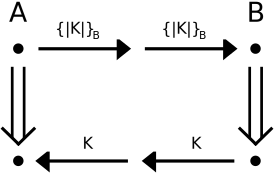
\includegraphics[width=0.5\textwidth]{half-duplex}
			\caption{
				A visual representation of the half-duplex protocol modeled in strand space
				\label{fig:half-duplex}
			}
		\end{figure}

		The geometric logic rules that model this protocol were generated
		manually by direct translation into geometric logic. Ideally, the
		process of generating geometric logic formul{\ae} from protocols should
		be done automatically.

	\subsection{The Results}

		The chase was run on the logic representation of the half-duplex protocol.
		A single model was returned during the execution of the algorithm,
		which was manually stopped before natural completion. This model,
		visualized in Figure \ref{fig:half-duplexCompleted}, like all models
		returned by the chase, satisfies the input theory, and belongs to a set
		of jointly minimal models for the theory.

		\begin{figure}[h]
			\centering
			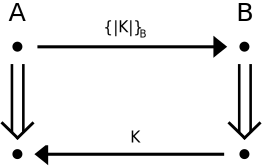
\includegraphics[width=0.5\textwidth]{half-duplexCompleted}
			\caption{
				A visual representation of the discovered run of the half-duplex protocol
				\label{fig:half-duplexCompleted}
			}
		\end{figure}

		The returned model denotes a run of the protocol which contains no
		adversary strands and is a correct execution of the protocol.
